\chapter{Theoretical Background} \label{chap:theoretical}

\section{Forecasting Models}
This Section details the forecasting models employed in each application described in Chapter \ref{chap:realworld}.


\subsection{Artificial Neural Networks}
\ac{ANN} is a computational model inspired by the structure and function of biological neural networks \cite{haykin1999Neural}. \ac{ANN}s consist of interconnected processing units, known as artificial neurons, that are organized into layers. Each artificial neuron receives inputs, performs a simple mathematical operation, and outputs a signal to other neurons in the network.

The inputs to the artificial neuron are multiplied by weight coefficients, which are then summed and passed through a non-linear activation function to produce the output. This output is then used as input to other neurons in the network.

\ac{ANN}s are trained by adjusting the weight coefficients through a process called error \ac{BP} \cite{bengio2016Deep}. \ac{BP} is an iterative optimization process that adjusts the weights based on the difference between the predicted output, and the actual target output \cite{haykin1999Neural}. This process is repeated until the prediction error is minimized, resulting in a trained \ac{ANN} \cite{bengio2016Deep}.

The architecture of an \ac{ANN} can vary, but common architectures include Feedforward Neural Networks, \ac{RNN}, and Convolutional Neural Networks. Feedforward Neural Networks consist of an input layer, one or more hidden layers, and an output layer. \ac{RNN} add feedback connections to feedforward neural networks, allowing the network to model temporal dependencies. Convolutional Neural Networks are specialized networks that process data with grid-like structures, such as images.

\subsubsection{Bayesian Regularized Neural Network}
\ac{BRNN} is a probabilistic extension of feedforward \ac{ANN}s that aims to address the issue of overfitting in traditional neural networks \cite{mackay1992Bayesian}. Overfitting occurs when the model is overly complex and captures noise in the training data, leading to poor generalization performance on unseen data.

\ac{BRNN} addresses this issue by incorporating a Bayesian framework into the training process, where the model parameters are treated as random variables with prior distributions. The network parameters are then optimized by minimizing the negative log-posterior probability of the model parameters given the data, which can be seen as a form of regularization. This results in a more robust and generalizable model compared to traditional neural networks \cite{mackay1992Bayesian, burden2008Bayesian}. According to \citeonline{zhou2022Determination}, the performance function of \ac{BRNN} can be represented as

\begin{equation}
    F = \alpha E_W + \beta E_D,
\end{equation}
where $E_W$ is the mean square of all the weights, $E_D$ is the mean square of prediction errors, $\alpha$ and $\beta$ are regularization coefficients. Further, Bayesian regularization assumes that the prior probabilities of the training dataset and weight parameters obey Gaussian distribution, adaptively optimizes the network weight parameters according to the Bayesian criterion, and determines $\alpha$ and $\beta$ at the minimum point of the improved performance function by maximizing the posterior probabilities \cite{zhou2022Determination}. Moreover, $\alpha$ and $\beta$ are given by

\begin{equation}
    \begin{cases}
        \alpha = \gamma / \left(2E_W\right) \\
        \beta = \left(N - \gamma\right) / \left(2E_D\right)
    \end{cases}
\end{equation}
where $N$ is the total number of samples, and $\gamma$ is the number of effective weights that can effectively reduce the training error, given by

\begin{equation}
    \gamma = N_W - 2\alpha tr\left(H^{-1}\right),
\end{equation}
where $N_W$ is the total number of the weight values and $H$ is the Hessian matrix of the performance function $F$, which can be simplified by the Gauss-Newton approximation \cite{mackay1992Bayesian}:

\begin{equation}
    H = \nabla^2 F \approx \alpha \nabla^2E_W + \beta \nabla^2E_D
\end{equation}

\subsubsection{Echo State Network}
\ac{ESN} were proposed by \citeonline{jaeger2001Echo} but became better known in 2004 through an article by the same author \cite{jaeger2004Harnessing}. \ac{ESN} is a \ac{RNN} with sparse connections within the internal layer, with random weights assigned to those connections. Input layer weights are typically assigned on a random basis. Usually, the output layer is trained, making this optimization problem far simpler. The training can be done using the Moore–Penrose pseudoinverse or with \citeonline{tikhonov1995Regularization} regularized regression (\ac{RIDGE}) \cite{tikhonov1995Regularization}. Fig.~\ref{fig:esn} shows a diagram of the \ac{ESN}.

\begin{figure}[!htb]
    \centerline{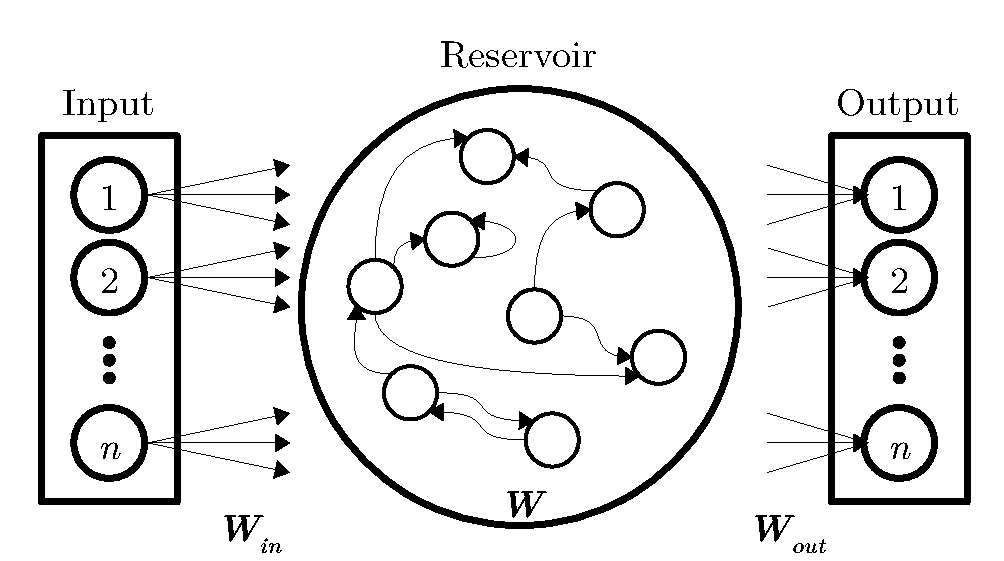
\includegraphics[width=0.8\linewidth]{Media/ESN_en.pdf}}
    \caption{Diagram of an ESN}
    \label{fig:esn}
    \source{\citeonline{larcher2021Forecasting}}
\end{figure}

The main parameters of the reservoir are, according to \citeonline{lukosevicius2012Practical}:

\begin{itemize}
    \item \textbf{Sparsity}: relates to how many random connections are in the reservoir, the ratio of zero elements over the total in the weights matrix.
    \item \textbf{Spectral radius} ($\rho$): the scaling factor of reservoir weights.
    \item \textbf{Size}: the number of neurons in the reservoir.
\end{itemize}

The \ac{ESN} usually also has a leaking rate ($\alpha$), which determines how much a past state influences the value of the next state in time. To define the \ac{ESN} when using \ac{RIDGE} is also necessary a ridge or regularization parameter ($\lambda$) for the training of the output layer. The weights of the output layer $\mathbf{W}_{out}$ can be calculated by

\begin{equation}
    \mathbf{W}_{out} = \mathbf{\hat{Y}} \mathbf{X}^T \left( \mathbf{X} \mathbf{X}^T + \lambda \mathbf{I} \right)^{-1},
\end{equation}
where $\mathbf{\hat{Y}}$ is the matrix containing the known values $y_t$, $\mathbf{X}$ is the matrix with input values and reservoir states, and $\mathbf{I}$ is the identity matrix.

\subsubsection{Long Short-Term Memory Network}
\ac{LSTM}, first described by \citeonline{hochreiter1997Long}, is a kind of \ac{RNN} with a ``memory'' property. The vanishing gradient is a recurring problem in \ac{RNN} trained with \ac{BP} based on gradient descent. In contrast, the network weights are iteratively updated considering the derivative concerning the last step weight. The gradient can get consistently small, causing the weights not to have any difference in each update. \ac{LSTM} networks can overcome this problem by storing information from the last steps in a vector, acting as a memory slot \cite{aggarwal2018Neural}. Figure \ref{fig:lstm} details a basic \ac{LSTM} unity.

\begin{figure}[htb!]
    \centering
    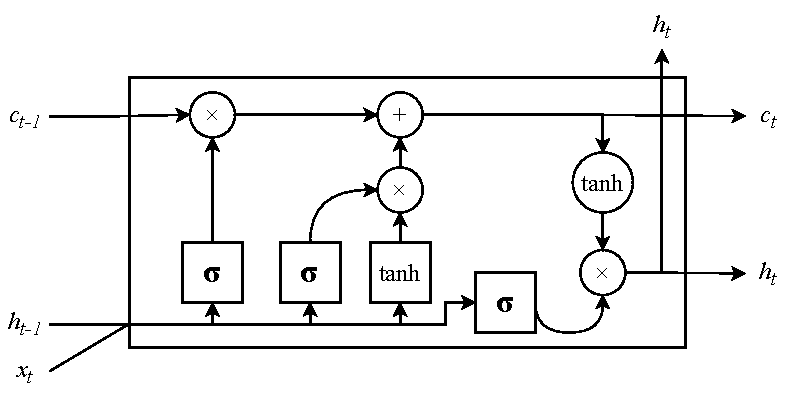
\includegraphics[width=0.8\linewidth]{Media/lstm.pdf}
    \caption{LSTM unity. Circles indicate point-wise operations, and squares indicate layers}
    \label{fig:lstm}
    \source{\citeonline{ribeiro2021Ensemble}}
\end{figure}

With $x_t$ as the update vector, $h_t$ as the hidden state vector, and $c_t$ the cell state, the updates for this unit are as follows, according to \citeonline{aggarwal2018Neural}, \citeonline{hochreiter1997Long}, and \citeonline{gers2000Learning}:

\begin{itemize}
    \item Input gate: \begin{equation}i_t = \sigma_{sigm}(W_{i} x_t + R_{i} h_{t-1} + b_i)\end{equation}
    \item Forget gate: \begin{equation}f_t = \sigma_{sigm}(W_{f} x_t + R_{f} h_{t-1} + b_f)\end{equation}
    \item Output gate: \begin{equation}o_t = \sigma_{sigm}(W_{o} x_t + R_{o} h_{t-1} + b_o)\end{equation}
    \item New cell state: \begin{equation}\tilde{c}_t = \sigma_{tanh}(W_{c} x_t + R_{c} h_{t-1} + b_c)\end{equation}
    \item Cell state selectively forgetting and adding to long-term memory: \begin{equation}c_t = f_t \odot  c_{t-1} + i_t \odot \tilde{c}_t\end{equation}
    \item Selectively leaking long-term memory to hidden state: \begin{equation}h_t = o_t \odot \sigma_{tanh}(c_t)\end{equation}
\end{itemize}
where $\sigma_{sigm}$ is a sigmoid activation function, $\sigma_{tanh}$ is a hyperbolic tangent activation function, $W$ is the weights matrix of the input vector, and $R$ is the matrix of weights of recurrent connections. Subscripts $i$, $f$, $o$, and $c$ indicate weights for the input, forget, output, and cell variables. Last, $b$ stands for the biases for the respectives gates.

\subsection{Cubist Regression}
\ac{CUBIST} is a rule-based algorithm used to build forecasting models (in the time series field) based on the analysis of input data \cite{quinlan1992Learning}. It estimates the target values by establishing regression models with one or more rules (committee/ensemble of rules) based on the input set. These rules are based on a combination of conditions with a linear function (generally linear regression). When the rule satisfies all conditions defined in the learning process, this approach can execute multiple rules once and find different linear functions. However, if the standard deviation reduction value is smaller or equal to the expected error for the sub-tree, some leaves are pruned to avoid overfitting \cite{ribeiro2020Shortterm}. 

\subsection{\textit{k}-Nearest Neighbors}
The \ac{KNN} is a non-parametric and instance-based method for classification and regression. Given a set of instances with known labels and a new instance to classify, the \ac{KNN} algorithm finds the $k$ nearest neighbors to the new instance and assigns the label that is most common among these neighbors \cite{altman1992Introduction}.

\ac{KNN} operates assuming that similar instances have similar labels. In other words, the closer two instances are in feature space, the more likely they will have the same label. Formally, let $ X$ represent the feature space, and the set of instances be represented by the set $x_1, x_2,\ldots, x_n$. For a new instance $x_{\text{new}}$, the distance between $x_{\text{new}}$ and $x_i$ is typically defined using a distance metric, such as the Euclidean distance:

\begin{equation}
    d\left(x_{\text{new}}, x_i\right) = \sqrt{\displaystyle \sum_{j=1}^m (x_{\text{new},j} - x_{i,j})^2}
\end{equation}
where $m$ is the number of features. The $k$ nearest neighbors to $x_{\text{new}}$ are the $k$ instances with the smallest distances to $x_{\text{new}}$. The label for $x_{\text{new}}$ is then determined by majority voting among the labels of the k nearest neighbors. The value of $k$ is an important hyperparameter in \ac{KNN} and is typically chosen through cross-validation. A small value of $k$, such as $k=1$, can result in overfitting, while a large value of $k$ can lead to underfitting.

\subsection{Partial Least Squares}
\ac{PLS} is a multivariate statistical method for analyzing the relationship between the response variables (the dependent variables) and the predictor variables (the independent variables). It is handy when the number of predictors (independent variables) is high relative to the number of observations, as it can reduce the dimensionality of the data while retaining important information \cite{wold1983Multivariate}.

Unlike traditional linear regression, \ac{PLS} forms latent variables that are linear combinations of the original variables. These latent variables capture the most important information in the predictors and the response variables. Let $X$ be a $n \times p$ data matrix, where $n$ is the number of observations, and $p$ is the number of predictors. Let $Y$ be a $n \times q$ data matrix, where $q$ is the number of response variables. The \ac{PLS} algorithm aims to find a set of latent variables, $T$, that can be used to approximate the relationship between $X$ and $Y$:

\begin{equation}
    \begin{cases}
            X \approx TP^T \\
            Y \approx UQ^T
    \end{cases}
\end{equation}
where $P$ and $Q$ are weighting matrices that represent the relationship between $X$ and $T$, and $Y$ and $U$, respectively.

\subsection{Quantile Random Forest}
\ac{QRF} \cite{meinshausen2006Quantile} is a tree-based machine learning approach that is an extension of the classical \ac{RF} algorithm \cite{breiman2001Random}. The main difference between \ac{QRF} and \ac{RF} is that \ac{QRF} is designed to predict the quantiles of a response variable instead of just its mean. This is achieved by modifying the way the terminal node predictions are made in each tree of the forest.

In \ac{RF}, the prediction for a terminal node is typically the average of the response values of the training samples that fall into that node. In contrast, \ac{QRF} predicts the quantile of the response values for each terminal node. Specifically, for a given quantile, the prediction for a terminal node is the quantile of the response values of the samples that fall into that node. The final prediction for a new sample is obtained by averaging the quantile predictions across all trees in the forest. 

\subsection{Regularized Regression}
Regularized regression is a type of regression analysis that aims to minimize the complexity of the model and prevent overfitting. Overfitting is a situation where a model fits too closely to the training data and, as a result, fails to generalize well to new unseen data, leading to imprecise performance on future data \cite{hoerl1970Ridge}.

\ac{RIDGE}, also known as Tikhonov regularization, is one of the most commonly used forms of regularized regression. It is used when the number of predictors in a dataset is larger than the number of observations. The goal of \ac{RIDGE} is to find the linear regression coefficients that minimize the sum of the squared residuals and the magnitude of the coefficients \cite{hoerl1970Ridge}. The mathematical formulation of \ac{RIDGE} can be represented as

\begin{equation}
    \beta_{\text{ridge}}=(X^TX + \lambda I)^{-1}X^Ty,
\end{equation}
where $\beta_{\text{ridge}}$ is the vector of regression coefficients, $X$ is the design matrix, $y$ is the vector of response variables, $\lambda$ is the regularization parameter, and $I$ is the identity matrix. The regularization parameter $\lambda$ controls the amount of regularization applied to the model. A larger value of $\lambda$ results in a more heavily regularized model, which can lead to smaller coefficients and a reduced risk of overfitting. On the other hand, a smaller value of $\lambda$ results in a less regularized model, which may overfit the data. The choice of the regularization parameter $\lambda$ can be determined through cross-validation or by using information criteria such as the Akaike Information Criterion or the Bayesian Information Criterion \cite{hoerl1970Ridge}.

\subsection{Stacking-Ensemble Learning}
\ac{STACK} is a methodology based on the divide-and-conquer principle. In this aspect, several base-learners (weak) are combined (by average rule for regression problems) to build an efficient model \cite{mendes-moreira2012Ensemble}. 

The \ac{STACK}-based ensemble learning improves accuracy by integrating many diverse base learners and operates using layers. Base learners are trained in the first layer (layer-0), and their predictions are used in the next layer. In the sequence, a meta-learner (layer-1) is trained, whose predictions of the previous layer are adopted as inputs, and predictions are obtained. The effectiveness of this methodology and the main advantage lies in the fact that different models can produce different predictions, and the meta-learner learns with these results.

The \ac{STACK} method improves forecasting output due to possible variance reduction of forecast error or correction of biases. Results from this learning process tend to converge for an improved solution compared to the base-learners \cite{wolpert1992Stacked}. A disadvantage of this approach is associated with the number of base learners used. However, the adoption of general-purpose machine learning wrappers freely available may overcome this by testing many different base learners as the syntax is unified.

Further, the improvement in the forecasting results occurs when there is diversity between the models of different levels, primarily due to models with varying principles of generalization tending to yield different results. In other words, the overall number of models in the layers does not guarantee the model performance, but its diversity \cite{ribeiro2020Ensemble}.

\subsection{Support Vector Regression}
\ac{SVR} is a generalization for regression of a supervised learning group called \ac{SVM} \cite{awad2015Support}. As described by \citeonline{drucker1997Support}, given a ``truth'' function $g(\boldsymbol{x})$ which is unknown in $d$-dimensional space and $f(\boldsymbol{x}, \boldsymbol{w})$ a family of functions defined by parameters $\boldsymbol{w}$, $\boldsymbol{\hat{w}}$ is the vector that minimizes the error between $g(\boldsymbol{x})$ and $f(\boldsymbol{x}, \boldsymbol{w})$. If $f_1(\boldsymbol{x}, \boldsymbol{\hat{w}})$ is a \ac{SVR} representation such as described by \citeonline{cortes1995Supportvector}:

\begin{equation}
    f_1(\boldsymbol{x}, \boldsymbol{\hat{w}}) =
    \sum_{i=1}^n (\boldsymbol{\alpha}_i^* - \boldsymbol{\alpha}_i)
    (\boldsymbol{\nu}_i^t \boldsymbol{x} + 1)^p +b
\end{equation}
where $\boldsymbol{\alpha}_i^*$ and $\boldsymbol{\alpha}_i$ and $b$ are constants of the model, $\boldsymbol{\nu}_j$ ($j = 1, 2, ..., n$) is the $j$-th training instance, $\boldsymbol{x}$ is the input space ($[x_1, x_2, ..., x_d]$) . The optimal values for $\boldsymbol{\hat{w}}$, $\alpha_i$ and $\alpha_i^*$ can be found by minimizing:

\begin{equation}
    U \sum_{i=j}^n L\{ y_j - F(\boldsymbol{\nu}_j, \boldsymbol{\hat{w}}) \} + || \boldsymbol{\hat{w}} ||^2
\end{equation}
where $L$ is a loss function and $U$ a regularization constant. Using this formulation with $L$ being the $\epsilon$-insensitive loss function \cite{cortes1995Supportvector} can solve the unknowns.

According to \citeonline{drucker1997Support}, this way, predictions $\boldsymbol{y}^{(p)}$ will take the form of:

\begin{equation}
    \boldsymbol{y}^{(p)} = 
    \sum_{i=1}^n (\boldsymbol{\alpha}_i^* - \boldsymbol{\alpha}_i)
    (\boldsymbol{\nu}_i^t \boldsymbol{x}^{(p)} + 1)^p +b
\end{equation}

One of the main advantages of \ac{SVR} lies in its capacity to capture the predictor non-linearity and then use it to improve the forecasting cases \cite{drucker1997Support}.

% \newpage
\section{Decomposition Methods}

\subsection{Complete Empirical Ensemble Mode Decomposition}
The \ac{CEEMD} is a data analysis method used to decompose a complex signal into its \ac{IMF} \cite{zhang2021Combined}. \ac{CEEMD} is an extension of the \ac{EMD} algorithm \cite{huang1998Empirical} and is designed to address the mode mixing problem in \ac{EMD}. This mode mixing occurs when the \ac{EMD} algorithm fails to accurately separate the \ac{IMF}s from the original signal, leading to inaccurate results. \ac{CEEMD} overcomes this problem by applying \ac{EMD} multiple times to the original signal, each time adding white noise to the input to create an ensemble of \ac{IMF}s \cite{zhang2021Combined}.

A short description of the \ac{CEEMD} process for an undecomposed input $y(t)$, is presented below by \citeonline{ali2020Complete}:

\begin{enumerate}
    \item Supply some white noise $\omega(t)$ to the time series ($x(t)$) such that $x'(t) = x(t) + \omega(t)$.

    \item Decompose $x'(t)$ via \ac{EMD} technique to obtain the first decomposed component.

    \item Follow steps 1 and 2 with a different number of realizations. This process is usually repeated with `$\tau$' numbers of times (ensemble number), each with various realizations.

    \item Then computing the mean of all IMF$_1$ as below:
    \begin{equation}
        \text{IMF}_1(t) = \frac{1}{\tau} \sum^\tau_{k=1} \psi_1 \left(x(t) + \varepsilon.\omega_k(t)\right),
    \end{equation}
where $\psi_1$ is the computation of $k^{th}$ IMF and $\varepsilon$ specifies the amplitude regulation necessary to obtain an appropriate signal.

    \item Hence, the first residual component or the remaining component results as follows:

    \begin{equation}
        R_1(t) = x(t) - \text{IMF}_1(t)
    \end{equation}

    \item Next, the extraction of IMF$_2$ from the original signal, $x(t)$, can be extracted as:

    \begin{equation}
        \text{IMF}_2(t) = \frac{1}{\tau} \sum^\tau_{k=1} \psi_1 \left[ x(t) + \varepsilon.\psi_1 \left( \omega_k(t) \right) \right]
    \end{equation}

    \item The above steps are repeated to acquire the $(\beta + 1)^{th}$ \ac{IMF} factor as:

    \begin{equation}
        \text{IMF}_{\beta+1}(t) = \frac{1}{\tau} \sum^\tau_{k=1} \psi_1 \left[ x(t) + \varepsilon.\psi_\beta \left( \omega_k(t) \right) \right]
    \end{equation}

    \item Finally, the residuals are averaged, which generally is the trend, displaying a gradual variation around the long-term average.
\end{enumerate}

\subsection{Singular Spectrum Analysis}
\ac{SSA} is a time series analysis and preprocessing technique. Its main objective is to identify significant components. \ac{SSA} is divided into two main parts: decomposition and reconstruction \cite{golyandina2001Analysis, moreno2018Wind, moreno2020Multistep}. The decomposition stage has the steps described as follows.

\begin{enumerate}

\item \textbf{Embedding}. Embedding consists in turning the one-dimensional time series into a high-dimensional matrix. So, given a time series in the form of $\boldsymbol{x}=\left\{ x_{1},x_{2},...,x_{N}\right\}$, it is possible to create a matrix $X$ of lagged vectors with a embedding dimension of $L$ in the following form:
%
\begin{equation}
X=\left[\begin{array}{ccccc}
x_{1} & x_{2} & x_{3} & \cdots & x_{K}\\
x_{2} & x_{3} & x_{4} & \cdots & x_{K+1}\\
x_{3} & x_{4} & x_{5} & \cdots & x_{K+2}\\
\vdots & \vdots & \vdots & \ddots & \vdots\\
x_{L} & x_{L+1} & x_{L+2} & \cdots & x_{N}
\end{array}\right]
\end{equation}
where the columns of $X$ are lagged vectors, $L$ is the dimension of the lagged vectors, and $K$ is the number of lagged vectors, with $K=N-L+1$.

\item \textbf{Singular Value Decomposition}. In this step the \ac{SVD} of the embedding matrix $X$ is computed, decomposing $X$ in $d$ components, in the form: $X=X_{1}+X_{2}+...+X_{d}$, where $d=\text{min}\left\{ L,K\right\}$. With $S=XX^{T}$, $\lambda_{i}$ are the eigenvalues of $S$. So, $X_i$ is correspondent with a $\lambda_{i}$ and can be written as: $X_{i}=\sqrt{\lambda_{i}}U_{i}V_{i}^{T}$, with $i\in\{1,2,...,d\}$, $U_{i}$ are the corresponding eigenvectors of $\lambda_{i}$, and $V_{i}=\frac{X^{T}U_{i}}{\sqrt{\lambda_{i}}}$. This set of $\{U_{i},\lambda_{i},V_{i}\}$ is called an eigentriple.

\end{enumerate}

The reconstruction stage has the following steps:

\begin{enumerate}
\item \textbf{Grouping}. In this step the set of eigentriples with indices $\{1,2,...,d\}$ are grouped into $m$ disjoint sets $I_{1},I_{2},...,I_{m}$. For each set $I_{j}$ has a corresponding $X_{Ij}$, that is the sum of every corresponding $X_{i}$ in the set.

\item \textbf{Diagonal averaging}. Every $X_{Ij}$ matrix is transformed in a series with length $n$. The process is called diagonal averaging, and for a matrix $Y$ with $L$ rows and $K$ columns, the construction of the series $\boldsymbol{y}$ has the following process. With $y_{ij}$ the element in the $i$ line in the $j$ column, let $L^{*}=\text{min}\{L,K\}$, $K^{*}=\text{max}\{L,K\}$, $y_{ij}^{*}=y_{ji}$ if $m<L$ or $y_{ij}^{*}=y_{ij}$ if $L<m$. Diagonal averaging is done with the following form:

\begin{equation}
y_{k}=\begin{cases}
\frac{1}{k}\sum_{m=1}^{k}y_{m,k-m+1}^{*}, & 1\le k\le L^{*}\\
\frac{1}{L^{*}}\sum_{m=1}^{L^{*}}y_{m,k-m+1}^{*}, & L^{*}\le k\le K^{*}\\
\frac{1}{N-k+1}\sum_{m=k-K^{*}+1}^{N-K^{*}+1}y_{m,k-m+1}^{*}, & K^{*} \le k\le N
\end{cases}.
\end{equation}

Applying it for all $X_{Ij}$ each $x_{Ij}$ is a component of the original time series $\boldsymbol{x}$.

\end{enumerate}

\subsection{Variational Mode Decomposition}
\ac{VMD}, introduced by \citeonline{dragomiretskiy2014Variational}, is a decomposition method that extracts a predetermined number $k$ of components from a time series. So given that the original time series signal is $g(t)$, \ac{VMD} subdivides it into $k$ signals $v_i$ in the form
%
\begin{equation}
    g(t) = \sum^{k}_{i=1} v_i,
\end{equation}
so that every $v_i$ is a mode with compact bandwidth around a center frequency $\omega_i$. The decomposition method can then be described with the following steps:

\begin{enumerate}
    \item Calculate the analytical signal of every $v_i$ using the Hilbert transform.
    \item Every mode is shifted by mixing it with an exponential with a frequency equal to the mode's center frequency.
    \item Calculate the demodulated signal's bandwidth utilizing a $L^2$-norm of the gradient (Gaussian smoothing).
\end{enumerate}

One of \ac{VMD} assumptions is that the original signal components are separated in frequency and are of narrowband. This premise makes \ac{VMD} less efficient when dealing with non-stationary wideband signals, especially with overlapping component spectra. This limitation is posed due to the difficulty of determining this type of signal's bandwidth. It has a large frequency content, and complex behavior for the overlapping modes, leading to poor physical interpretability \cite{moreno2020Multistep}. For more detailed steps, \citeonline{dragomiretskiy2014Variational}, \citeonline{moreno2020Multistep}, and \citeonline{moreno2021Hybrid} should be consulted.

% \newpage
\section{Preprocessing Techniques}
This section details the preprocessing approaches employed in each application described in Chapter \ref{chap:realworld}.

\subsection{Box-Cox Transformation}
The \ac{BC}, proposed by \citeonline{box1964Analysis}, is a statistical technique that aims to transform non-normally distributed data into a more normal-like distribution, which is more suitable for certain statistical methods. The transformation is defined by \citeonline{lyu2022Synchronous} as

\begin{equation}
    y(\lambda) =
        \begin{cases}
            \frac{y^{\lambda} - 1}{\lambda}, & \text{if } \lambda \neq 0 \\
            \log y, & \text{if } \lambda = 0
        \end{cases}
\end{equation}
where $y(\lambda)$ denotes the transformed data and $\lambda$ is a parameter that needs to be estimated. The value of $\lambda$ that optimizes the normality of the transformed data can be obtained through maximum likelihood estimation or graphical methods. The \ac{BC} has been used to make non-normally distributed data more suitable for regression analysis and other statistical methods that assume normality.

\subsection{Correlation Matrix}
A \ac{CORR} is a table that displays the pairwise correlations between variables in a dataset. The entries in the matrix are usually \ac{PCC}, which are measures of linear association between two variables \cite{benesty2009Pearson, kuhn2013Applied}. The \ac{PCC} can be defined as the covariance of the $a$ and $b$ (two variables) divided by the sum of their standard deviation \cite{pawan2023Electroencephalogram}, as

\begin{equation}
    \rho(a,b) = \displaystyle \sum^n_{i=1} \left(\frac{a_i-\bar{a}}{\sigma_a}\right) \left(\frac{b_i-\bar{b}}{\sigma_b}\right),
\end{equation}
where $\bar{a}$ and $\bar{b}$ are the means of variables $a_i$ and $b_i$, respectively, $\sigma_a$ and $\sigma_b$ the standard deviation of the two variables, and $n$ is the sample size. In the \ac{PCC}, the value of $\rho(a,b)$ ranges from -1 to 1, where -1 indicates a strong negative linear relationship, 1 indicates a strong positive linear relationship, and 0 indicate no linear relationship between the two variables.

\subsection{Principal Component Analysis}
\ac{PCA} is a dimensionality reduction technique widely used in pattern recognition, and machine learning \cite{wold1987Principal}. \ac{PCA} is a linear method that transforms a set of correlated variables into a set of uncorrelated variables, known as principal components, which capture the maximum variability in the data \cite{jackson1991User}.

Given a set of $n$ observations, $X={x_1,x_2, \dots, x_n}$, where each $x_i$ is a $d$-dimensional vector, \ac{PCA} seeks to find the linear combination of variables that capture the most variation in the data. To achieve this, \ac{PCA} finds the eigenvectors of the covariance matrix of $X$, denoted by $Cov(X)$, and orders them by the magnitude of their corresponding eigenvalues. The eigenvectors with the largest eigenvalues are chosen as the principal components, and the data is projected onto these components \cite{wold1987Principal}. \ac{PCA} has several advantages, such as removing the noise and reducing the complexity of the data, allowing for more straightforward interpretation and visualization. It is also widely used to preprocess data before applying more complex machine learning algorithms.

% \newpage
\section{Performance Measures}
Different performance metrics are utilized to evaluate the presented models and compare them to other models. The chosen performance metrics were the \ac{IP}, \ac{MAE}, \ac{MAPE}, \ac{RMSE}, \ac{RRMSE}, \ac{sMAPE}, and \ac{SSE}. The metrics are calculated using the test set with out-of-sample values. Each metric is defined as follows:

\begin{equation}
    \textnormal{IP} = \frac{M_c - M_b}{M_c} \times 100,
    \label{eq:ip}
\end{equation}
\begin{equation}
    \textnormal{MAE} = \frac{1}{n} \displaystyle \sum_{i=1}^{n} \left|y_{i}-\hat{y}_{i}\right|,
    \label{eq:mae}
\end{equation}
\begin{equation}
	\textnormal{MAPE} = \frac{1}{n}\displaystyle \sum_{i=1}^{n}\left|\frac{y_{i}-\hat{y}_{i}}{y_{i}}\right|\times 100,
	\label{eq:mape}
\end{equation}
\begin{equation}
	\textnormal{RMSE} = \displaystyle \sqrt{\frac{1}{n}\sum_{i=1}^{n} (y_i-\hat{y}_i)^2},
	\label{eq:rmse}
\end{equation}
\begin{equation}
	\textnormal{RRMSE} = \frac{\sqrt{\frac{1}{n} \displaystyle \sum_{i=1}^{n} \left(y_i-\hat{y}_i\right)^2}}{\frac{1}{n} \displaystyle \sum_{i=1}^{n} y_i},
	\label{eq:rrmse}
\end{equation}
\begin{equation}
    \textnormal{sMAPE} = \frac{2}{n} \displaystyle \sum_{i=1}^{n} \frac{\left|y_i - \hat{y}_i\right|}{\left|y_i\right|+\left|\hat{y}_i\right|},
    \label{eq:smape}
\end{equation}
\begin{equation}
    \textnormal{SSE} = \displaystyle \sum_{i=1}^{n} \left(y_i - \hat{y}_i\right)^2,
    \label{eq:sse}
\end{equation}
where $n$ is the number of observed samples, $y_i$ is the $i$-th measured real value, and $\hat{y}_{i}$ is the $i$-th predicted value. Also, $M_c$ is the performance of the compared model, $M_b$ is the performance of the best model, and can be \ac{MAE}, \ac{MAPE}, \ac{RMSE}, \ac{RRMSE}, \ac{sMAPE}, and \ac{SSE}.

% \newpage
\section{Hypothesis Tests}
Moreover, the \ac{DM} test, proposed by \citeonline{diebold2002Comparing}, was performed to determine the significance of the difference in error in the analyzed forecasts. The \ac{DM} test verifies if the errors are significantly lower. The \ac{DM} test's null hypothesis ($H_0$) states that there is no difference between the errors of the compared methods, and the alternative hypothesis ($H_1$) states that the forecasting error of the proposed model is lower than compared one. The hypothesis test can be defined as follows,

\begin{equation}
    \begin{cases}
    \displaystyle  H_{0}: \epsilon^{P}_{i} = \epsilon^{C}_{i} \\
    \displaystyle  H_{1}: \epsilon^{P}_{i} < \epsilon^{C}_{i},
    \end{cases}
    \label{eq:DMH}
\end{equation}
where $\epsilon_{i}^{P} = y_i - \hat{y}_i^P$ and $\epsilon_{i}^{C} = y_i - \hat{y}_i^C$ are the error of the proposed and the compared model, respectively, $\hat{y}_i^P$ and $\hat{y}_i^C$ are the predictions of the proposed and compared models, respectively. The \ac{DM} test is based on the loss differentials $d_i$, given by

\begin{equation}
    d_i=\ell (\epsilon_{i}^P) - \ell (\epsilon_{i}^C),
    \label{eq:dmloss}
\end{equation}
where $\ell$ is a loss function that estimates the accuracy of each model. Then, let the sample mean loss differential, $\overline{d}$, be

\begin{equation}
    \overline{d} = 
    \frac{1}{n} \displaystyle \sum_{i=1}^{n} d_i =
    \frac{1}{n} \displaystyle \sum_{i=1}^{n} \left[ \ell (\epsilon_{i}^P) - \ell (\epsilon_{i}^C) \right].
    \label{eq:meanloss}
\end{equation}

The statistic of \ac{DM} test is given by

\begin{equation}
DM = \frac{\overline{d}}{\sqrt{\frac{2\pi\hat{f}_d(0)}{n}}}, \label{eq:DMS}
\end{equation}
where $2\pi\hat{f}_d(0)$ is a consistent estimator of the asymptotic variance of $\sqrt{nd}$.

The defined hypothesis test evaluates whether the errors for a given model are smaller than those of a compared model. When the null hypothesis is rejected, the errors of a model (proposed model) concerning another (comparison) have been reduced with a given significance level.